\documentclass{amsart}
\usepackage[utf8]{inputenc}
\usepackage{enumerate}
\usepackage{graphicx}

\usepackage{a4wide}

\theoremstyle{definition}
\newtheorem{problem}{Problem}

\title{\sc Logic Tutorial: Worksheet 2}

\date{}


\begin{document}

\maketitle

\subsection*{Topics:} Theories. Normal forms, CNF and DNF, SAT and 3-SAT.  3-SAT. 2-SAT and implication graph, Horn-SAT and unit propagation. Encoding problems in SAT.

\bigskip

\hrule

\bigskip\begin{problem}
Consider the propositional theory $T=\{\neg q \to (\neg p \vee q),\ \neg p \to q,\ r \to q\}$ over the language $\{p, q, r, s\}$. Which of the following propositions are valid, contradictory, independent, satisfiable, equivalent in $T$?
\begin{enumerate}[(a)]
\item $p$, $q$, $r$, $s$, $\neg p$, $\neg s$
\item $p \vee q$,\ $p \vee r$,\ $p \vee s$,\ $q \vee s$
\item $p \wedge q$,\ $q \wedge s$,\ $p \to q$,\ $s \to q$
\end{enumerate}
\end{problem}


\hrule


\bigskip\begin{problem} Given a formula $\varphi$ in CNF or DNF, A) count the number of models and B) describe all its models.
\begin{enumerate}[a)]
\item $(p_1 \wedge  \neg p_2 \wedge  p_3 \wedge  \neg p_4 )\vee(p_2 \wedge  p_3 \wedge  \neg p_4 )\vee(\neg p_3)\vee(p_2 \wedge  p_4)\vee(p_1 \wedge  p_3 \wedge  p_5 )\vee(p_3 \wedge  \neg p_4 \wedge  p_2 )$
\item $(p_1 \vee \neg p_2 \vee p_3 \vee \neg p_4 )\wedge(p_2 \vee p_3 \vee \neg p_4 )\wedge(\neg p_3)\wedge(p_2 \vee p_4)\wedge(p_1 \vee p_3 \vee p_5 )\wedge(p_3 \vee \neg p_4 \vee p_2 )$
\end{enumerate}
\end{problem}


\bigskip\begin{problem} Transform the following propositional formulas into CNF and DNF A) using truth tables (determining models), B) using syntactic rules:
\begin{enumerate}[a)]
    \item $(\neg p \vee q)\to (\neg q \wedge r)$,
    \item $(\neg p \to (\neg q \to r))\to p$,
    \item $((p\to \neg q) \to \neg r) \to \neg p$.
\end{enumerate}
\end{problem}


\bigskip\begin{problem} Given a formula $\varphi$ in CNF, find a 3-CNF formula $\varphi'$ such that $\varphi'$ is satisfiable iff $\varphi$ is satisfiable. Describe an efficient algorithm to construct $\varphi'$ given $\varphi$ (a reduction from SAT to 3-SAT).
\end{problem}


\bigskip\begin{problem} Find the (shortest possible) CNF and DNF representations of the Boolean majority function $\mathrm{maj}: {^3}2\to 2$ which outputs the majority vote of the input values.
\end{problem}


\bigskip\begin{problem} Can you find CNF and DNF representations of the Boolean $n$-ary parity function $\mathrm{par}: {^n}2\to 2$ defined by $\mathrm{par}(x_1,\dots,x_n)=(x_1+\dots+x_n)\bmod 2$
which outputs the XOR of all input values? Try it for small values of $n$.
\end{problem}

\bigskip\begin{problem} Let $\mathbb P$ be a countably infinite set of propostional letters. Show that it is no longer true that every $K\subseteq {^\mathbb P}2$ can be modelled by both a CNF and a DNF formula. Find such a set of models $K$ which cannot be modelled by either.
\end{problem}


\hrule


\bigskip\begin{problem} Construct the implication graph of the following 2-CNF formula. Is the formula satisfiable? If it is, find a solution.
\begin{enumerate}[a)]
\item $(p_1\vee \neg p_2)\wedge (p_2\vee p_3)\wedge (\neg p_3\vee \neg p_1)\wedge (\neg p_3\vee \neg p_4)\wedge (p_4\vee p_5)\wedge (\neg p_5\vee \neg p_1)$,
\item $(p_1\vee \neg p_2)\wedge (p_2\vee p_3)\wedge (\neg p_3\vee p_1)\wedge (\neg p_3\vee \neg p_4)\wedge (p_4\vee p_5)\wedge (\neg p_5\vee p_1)$,
\item $(p_0 \vee  p_2) \wedge  (p_0 \vee  \neg p_3) \wedge  (p_1 \vee  \neg p_3) 
\wedge  (p_1 \vee  \neg p_4) \wedge  (p_2 \vee  \neg p_4) 
\wedge  (p_0 \vee  \neg p_5)
\wedge 
(p_1 \vee  \neg p_5) \wedge  (p_2 \vee  \neg p_5) \wedge  (\neg p_1 \vee  \neg p_6) \wedge  (p_4 \vee  p_6) \wedge  (p_5 \vee  p_6) \wedge  p_1\wedge \neg p_7$.
\end{enumerate}
\end{problem}

\bigskip\begin{problem}
Apply the unit propagation algorithm to determine whether the following Horn formula is satisfiable. It it is, find a satisfying assignment.
\begin{align*}
&(\neg p_1 \vee \neg p_3 \vee p_2)\wedge(\neg p_1 \vee p_2)\wedge p_1 \wedge (\neg p_1 \vee \neg p_2 \vee p_3)\wedge \\
&(\neg p_2 \vee \neg p_4 \vee p_1)\wedge(\neg p_4 \vee \neg p_3 \vee \neg p_2)\wedge(p_4\vee \neg p_5 \vee\neg p_6)
\end{align*}
\end{problem}



\hrule









% \bigskip\begin{problem}
% Let $\mathrm{maj}_n: {^3}({^n}2)\to {^n}2$ be the coordinate-wise majority function, that is, for example
% $$
% \mathrm{maj}_4((0, 1, 0, 1),(1, 1, 0, 0),(1, 1, 0, 0)) = (1, 1, 0, 0).
% $$
% We say that a set $K\subseteq {^n}2$ is a \emph{median set} if it is closed under $\mathrm{maj}_n$.
% \begin{enumerate}[a)]
%     \item Show that for every 2-CNF propositional formula $\varphi$, $M(\varphi)$ is a median set.
%     \item* Show that for every median set $K\subseteq {^n}2$ there exists a 2-CNF formula $\varphi$ over $n$
% variables such that $M(\varphi) = K$.
%     %\item** What about the coordinate-wise $n$-ary parity function?
% \end{enumerate}
% \end{problem}






\bigskip\begin{problem}
Can a $4\times 4$ chessboard with two opposite corners removed be perfectly covered by domino tiles? Encode the problem as a SAT formula. Generalize to all even $n$.
\end{problem}



\bigskip\begin{problem}
Can you color integers from 1 to $n$ with two colors so that the equation $a+b=c$ has no monochromatic solutions with $1\leq a<b<c\leq n$? Construct a CNF formula $\varphi_n$ which is satisfiable, if and only if such a coloring is possible. Try $n=8$ first.

Try this at home: Write a script generating $\varphi_n$ in DIMACS CNF format. Use a SAT solver to find the smallest $n$ for which no such coloring exists (i.e., any 2-coloring has a monochromatic triple $a<b<c$ with $a+b=c$).
\end{problem}



\bigskip\begin{problem}
Encode the problem of sorting three integer numbers in SAT.
\end{problem}



\bigskip\begin{problem}
The famous Four Colour Theorem says that the following map can be colored by 4 colors so that no two adjacent regions share the same colour. Find such a coloring (using a SAT solver).
\begin{center}
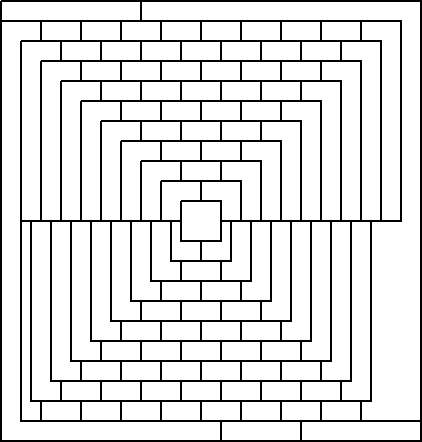
\includegraphics[width=0.8\textwidth]{files/map.png}
\end{center}
\end{problem}

\end{document}
